\documentclass[letterpaper, 10 pt, conference]{ieeeconf}

%\let\labelindent\relax
%\IEEEoverridecommandlockouts
%\overrideIEEEmargins

%floats and figures
\usepackage{graphics}
\usepackage[pdftex]{graphicx}
\usepackage[font={small}]{caption}
\usepackage{subcaption}
%\usepackage[center]{subfigure} %DONT USE BOTH SUBCAPTION AND SUBFIGURE
%\DeclareGraphicsExtensions{.pdf,.png,.jpg}
%\usepackage{overpic}
%\usepackage[rightcaption]{sidecap}
%\usepackage{pbox}

%Math Stuff
\usepackage{mathtools}
\usepackage{amsmath, amssymb, amscd}
%\usepackage{ wasysym } %special symbols
\usepackage{amsfonts}
\usepackage{mathptmx}       % selects Times Roman as basic font
\DeclareMathAlphabet{\mathcal}{OMS}{lmsy}{m}{n}
\DeclareSymbolFont{largesymbols}{OMX}{cmex}{m}{n}
\usepackage{algorithm}
\usepackage{algorithmicx}
%\usepackage{algorithm}
%\usepackage{algpseudocode}
% \usepackage[ruled,vlined,linesnumbered]{algorithm2e}
\usepackage{ textcomp } %for getting text tilde

%Table Stuff
\usepackage{array} %for table entries to be in center of cell
\usepackage{tabularx}
\usepackage{multicol}
\usepackage{multirow}

%DOCUMENT WIDE
\usepackage{times} % assumes new font selection scheme installed
\usepackage{xspace}
\usepackage[english]{babel} %for hyphenation rules
%\usepackage{flushend}%balance columns on last page
\usepackage{fixltx2e} %fix latex issue across versions
\usepackage{bm}
\usepackage{units}

\usepackage{makeidx}
% \usepackage{enumitem}
\usepackage[yyyymmdd,hhmmss]{datetime}
\usepackage[english]{babel}

%Bibliography and cross-ref
\makeatletter
\let\NAT@parse\undefined
\makeatother
\usepackage[numbers]{natbib}
\renewcommand{\bibfont}{\footnotesize}
% \usepackage{cite} %DONT USE NATBIB AND CITE TOGETHER

%hyperlinking
\usepackage{url}
\makeatletter
\g@addto@macro{\UrlBreaks}{\UrlOrds}
\makeatother
\usepackage{color}
\usepackage[usenames,dvipsnames, table]{xcolor}
\usepackage[pdfborder={0 0 0.5}]{hyperref}
\hypersetup{
    colorlinks=true,
    linkcolor=blue,
    citecolor=black,
    filecolor=cyan,
    urlcolor=blue
}


%=======U S E R  D E F I N E D  M A C R O S=======
% \newcommand{\bibhref}[2]{#2}
\newcommand{\todo}[1]{\textcolor{red}{[ToDo:#1]}}
\newcommand{\tocite}[1]{\textcolor{red}{[cite]}}
\newcommand{\ignore}[1]{}

% Usage:
% \figlabel{myfigure} creates \label{fig:myfigure}
% \figref{myfigure} references it
\newcommand{\figlabel}[1]{\label{fig:#1}}
\newcommand{\figref}[1]{Figure~\ref{fig:#1}}

% Usage:
% \seclabel{mysection} creates \label{sec:mysection}
% \secref{mysection} references it
\newcommand{\seclabel}[1]{\label{sec:#1}}
\newcommand{\secref}[1]{Section~\ref{sec:#1}}

% Usage:
% \tablabel{mytable} creates \label{tab:mytable}
% \tabref{mytable} references it
\newcommand{\tablabel}[1]{\label{tab:#1}}
\newcommand{\tabref}[1]{Table~\ref{tab:#1}}

% use this command instead of writing "da Vinci" so it's never split 
\newcommand{\davinci}{da~Vinci\xspace}

\usepackage{blindtext}

%===============================================================
\title{\LARGE \bf
Deep Segmentation of Surgical Robot Trajectories from Video 
}
% Pixels to Primitives (P2P)

\author{%
Adithyavairavan Murali, Animesh Garg, Sanjay Krishnan, Florian Pokorny, Ken Goldberg
%Authors are with the Department of Electrical Engineering and Computer Sciences, University of California at Berkeley, CA, USA.}
\thanks{$^{1}$EECS, University of California, Berkeley; {\{sanjaykrishnan, adithya\_murali\}@berkeley.edu}}%
\thanks{$^{2}$IEOR and EECS, University of California, Berkeley; {\{animesh.garg, goldberg\}@berkeley.edu}}%
}

\newcommand{\sys}{\textsf{DeepSeg}\xspace}

\begin{document}

\maketitle

\begin{abstract}
Segmentation is an important first step in analyzing long running robotic tasks. For reliable results, it is important to consider both visual and kinematic data, as visual data provides important information about the state of the workspace. 
Existing unsupervised segmentation methodologies are limited in the ways they can leverage visual data and rely on annotations or complete knowledge of all objects in the world. In this paper, we propose a framework that takes a step towards unsupervised segmentation of robotic demonstrations using raw video (i.e., pixel data). 
We identify key transition events in kinematic data, cluster transitions together using visual data, and then identify segments of the raw video corresponding to these clusters of transition events. 
The resulting video segments can be used to design error recovery actions, parameter tuning, action classification, 
and operator skill assessment. 
\todo{Our results on x suggest y}
\end{abstract} 

\section{Introduction}
Segmenting demonstrations of a multistep task is an important first step in a number of robot learning applications: skill-learning \cite{calinon2010learning, kruger2010learning, konidaris2011robot}, learning from demonstrations \cite{Niekum2015learning}, reward function parametrization \cite{hanlearning}, and automation of surgical subtasks \cite{murali2015learning}.
One approach is manual annotation, which can be time-consuming and error-prone if inconsistent.
Therefore, it is desirable to algorithmically extract segments from unlabled data.
Such algorithms fall into two broad categories: (1) dictionary-based, (2) and unsupervised.
Dictionary-based algorithms set a pre-defined vocabulary of primitives \emph{a priori} and decompose new trajectories in terms of the primitives; and this approach has been widely applied in the analysis of robotic surgery \cite{lea15improved,zappella2013surgical}.

However, the key challenge in using a dictionary-based approach is building the dictionary of primitives. 
Overly specific primitives may not cover all of the actions seen in a set of demonstrations, while overly general primitives may miss task-specific structure.
Unsupervised techniques can avoid dependence on a pre-defined set of primitives.
Unsupervised methods typically assume some generative mixture model for the data, e.g., locally Gaussian segments, and fit trajectories to this model grouping together locally similar points \cite{calinon2010learning, krishnan2015tsc, calinon2004stochastic, kruger2010learning, fox2009nonparametric, oh2005learning}.


\begin{figure}[ht]
\centering
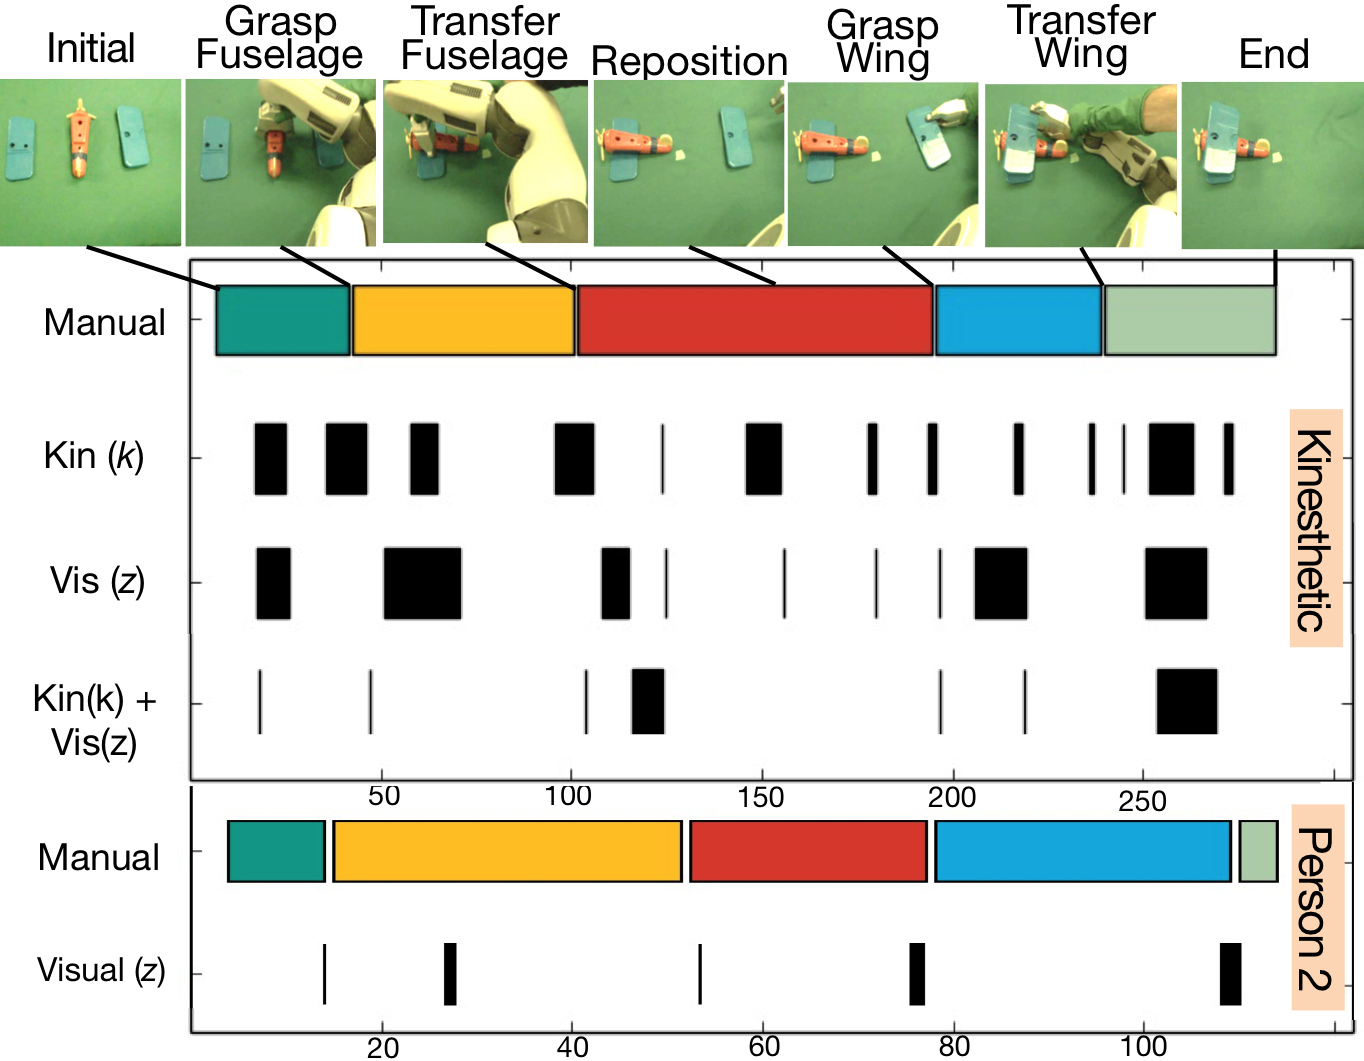
\includegraphics[width=\linewidth]{figures/pr2_plane_assembly.png}
\caption{The figure shows a sequence of images from the Toy Plane assembly (YCB Dataset). The first row shows a manual segmentation of the task in 4 semantic steps: Grasp Fuselage, Transfer Fuselage, Grasp Wing, Transfer Fuselage. Rows 2-4 show the sub-task level segmentation results from our completely unsupervised approach using 8 examples. Each row is a sequence of transitions represented by blocks. The width of every block represents the confidence interval conveying the length of transition, with some transitions being sharp while others are longer.}
 \label{fig:pr2_toyplane}
\vspace{-10pt} 
\end{figure}

While unsuperivsed segmentation has been widely studied in the context of kinematic data segmentation, increasingly, fixed camera video recordings accompany kinematic recordings of human teleoperation in a variety of datasets \cite{hodgins2009guide, gao2014jigsaws, ofli2013berkeley}.
The importance of visual sensing in segmentation has been suggested by experimental results in our prior work \cite{krishnan2015tsc} and by others \cite{Niekum2015learning}.
Visual features can provide crucial information in a number of scenarios: (1) a robot can only partially observe its state with kinematic data, (2) state-dependent sensor noise in a robots kinematic data, and (3) manipulations of objects in the environment.
However, existing unsupervised approaches rely on highly constrained visual sensing models: hand tuned features \cite{krishnan2015tsc}, poses for all objects in the workspace via AR markers \cite{Niekum2015learning}, or motion capture markers in human gesture extraction \cite{kulic2011incremental}.

In this work, we explore how we can relax these constraints by segmenting both kinematics and natural videos of demonstrations.
The key problem is leveraging raw visual data, i.e., pixels, due to the dimensionality and the featurization problem.
Fortunately, in computer vision, the growing maturity of \emph{deep} featurization e.g., Convolutional Neural Networks (CNNs), has led to a number of seminal results in visual feature extraction \cite{krizhevsky2012imagenet, lecun1995convolutional, jia2014caffe, long2014fully}.
Furthermore, frameworks like CAFFE \cite{jia2014caffe} allow for sharing pre-trained models (on terabyte-scale corpora of natural images), and this allows us to take advantage of these results even with relatively small datasets.

We explore an extension (\sys) to the Transition State Clustering algorithm \cite{krishnan2015tsc} with visual features.
At a high-level, this algorithm models demonstrations as switched linear dynamical systems.
It then identifies states at which regime transitions occur and clusters these states to identify regions of the state space associated with transitions.
The minimal covering set of transition clusters, i.e., clusters representing all demonstrations, gives a semantic segmentation for a task. 
We extend this framework by specifying the state space not only with kinematic states but also augmented with visual features.
Our experimental results surprisingly suggest that a time-series of frame-level visual features behave almost like smooth kinematic trajectories--satisfying the assumptions in our prior work.
Even with featurized videos, segmentation is not trivial, and there are a number of open questions including how to incorporate visual features into the model, how to navigate the number of hyperparameter and architecture choices, and the sufficiency of pre-trained networks.

We summarize the key experimental results.

\vspace{0.25em}

\textbf{Q0. Do generic visual features, deep or otherwise, improve segmentation accuracy? } While prior work in segmentation establishes that features from a constrained/hand-annotated visual sensing model can improve segmentation, an open question is whether there is enough information in natural videos with general-purpose features to improve segmentation accuracy. Our experimental results find that under partial kinematic observation and sensing noise, visual features dramatically improve segmentation accuracy by \textbf{x\%???}.

\vspace{0.25em}

\textbf{Q1. How do we transfer pre-trained neural network features to a very different domain? } Transfer learning of convolutional neural networks is an open problem in the computer vision community and a number of recent publications suggest caution or highly sensitive results \cite{oquab2014learning}.  These networks are trained on very different corpora of images than those seen in robotic demonstration videos. Even so, our results suggest that with the appropriate choice of convolutional layer to transfer, we can achieve accuracy improvements of \textbf{x\%???}.

\vspace{0.25em}

\textbf{Q2. How should visual features be incorporated into a kinematic segmentation model? } Even with automated featurization, the visual feature space is much higher dimensional than the kinematic state space. We explore dimensionality reduction techniques to mitigate some challenges due to the dimensionality. A natural approach would be to treat this problem as a multi-view manifold alignment problem e.g., finding a feature space maximally correlated with kinematics with Canonical Correlation Analysis. Surprisingly, our results suggest that this approach discards the novel information discovered by vision, and in fact random projections would do just as well (\textbf{x\%???}).

\vspace{0.25em}

\textbf{Q3. How do learned segmentations compare with human annotations? } We apply \sys to data from two datasets of surgical tasks \cite{gao2014jigsaws} where there were also human annotations of the same tasks.
While we find that \sys mostly agrees with the human annotations, there are a number of instances where \sys find crucial actions missed by the human annotators. (\textbf{List examples}) 

\iffalse
\begin{figure}[ht]
\centering
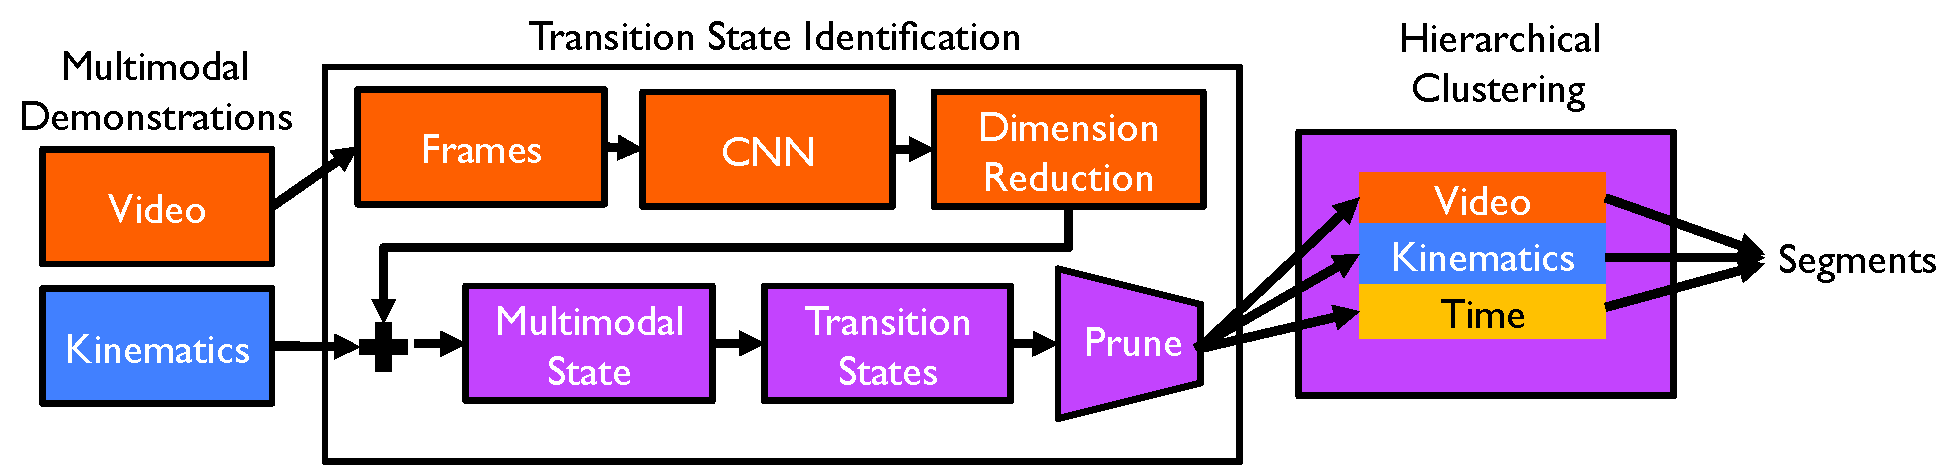
\includegraphics[width=\columnwidth]{figures/architecture.pdf}
\caption{\todo{name} architecture. We use a pre-trained CNN to featurize raw video data for use in segmentation. After featurization, we combine the data with kinematic data and apply a Transition State Clustering algorithm to identify segments. \label{fig:arch}}
\vspace{-1em}
\end{figure}
\fi

\section{Related Work}

\noindent\textbf{Surgical Segmentation: }

\begin{enumerate}
\item Describe ``surgeme" work
\end{enumerate}

\noindent\textbf{Segmentation in Other Robotics: }

\begin{enumerate}
\item Describe Neikum/others like DMP, GMM etc.
\end{enumerate}

\noindent\textbf{Related work in Computer Vision: }

\begin{enumerate}
\item Introduce Convolutional Network Research.
\end{enumerate}

\section{Problem Setup and Notation}
We first overview the Transition State Clustering algorithm.

\subsection{Transition State Clustering Model}
At a high-level, the Transition State Clustering algorithm (\sys), clusters states that mark dynamical regime transitions across all demonstrations.
This finds a discrete parametrization for transition events that can be used for segmentation.
In our prior work, we found that this model was more robust in comparison to alternatives.
We first outline the model, and then describe the algorithm to fit the parameters.

\subsubsection{Dynamical System Model}
Let $\mathcal{D}=\{d_i\}$ be the set of demonstrations where each $d_i$ is a trajectory $\mathbf{x}(t)=\binom{k(t)}{z(t)}$ of fully observed robot states and each state is a vector in $\mathbb{R}^d$.
$\mathbf{x}(t)$ encapsulates both the kinematic state $k(t)$ and a set of visual features $z(t)$.
We model each demonstration as a switched linear dynamical system.
There is a finite set of $d \times d$ matrices $\{A_1,...,A_k\}$, and an i.i.d zero-mean additive Gaussian Markovian noise process $W(t)$ which accounts for noise in the dynamical model:
\[
\mathbf{x}(t+1) = A_{i}\mathbf{x}(t) + W(t) \text{ : } A_i \in \{A_1,...,A_k\}
\]
In this model, transitions between regimes are instantaneous where each time $t$ is associated with exactly one dynamical system matrix $1,...,k$.

\subsubsection{Transition State Clusters}
Transition states are defined as the last states before a dynamical regime transition in \emph{each} demonstration.
Therefore, there will be times $t$ at which $A(t) \ne A(t+1)$.
A transition state is the state $x(t)$ at time $t$.
For a demonstration $i$, we denote the sequence of transitions states as $U_i=[u_i^1,...,u_i^J]$.
$J$ is the number of transition states where $J\ll T_i$ where $T_i$ is the time-length of $d_i$.

A \emph{transition state cluster} is
defined as a clustering of the set of transition states across all demonstrations; partitioning these transition states into $m$ non-overlapping similar groups:
\[
\mathcal{C} = \{C_1, C_2,...,C_m\}
\]
Every $U_i$ can be represented as a sequence of integers indicating that transition states assignment to one of the transition state clusters $U_i=[1,2,4,2]$.

We assume, demonstrations are \emph{consistent}, meaning there exists a non-empty sequence of transition states $\mathcal{U}^*$ such that the partial order defined by the elements in the sequence (i.e., $s_1$ happens before $s_2$ and $s_3$) is satisfied by every $U_i$. For example, 
\[U_1 = [1,3,4]\text{, }U_2 = [1,1,2,4]\text{, }\mathcal{U}^*=[1,4] \]
A counter example,
\[U_1 = [1,3,4]\text{, }U_2 = [2,5]\text{, }\mathcal{U}^*\text{  no solution} \]
Intuitively, this condition states that there have to be a consistent ordering of actions over all demonstrations up to some additional regimes (e.g., spurious actions). 
In case of multiple modes in an action sequence, we find the minimal consistent set.


\noindent \emph{Given a consistent set of demonstrations, the goal of the algorithm is to find a minimal solution, $\mathcal{U}^*$ that is loop free and respects the partial order of transitions in all demonstrations.}

\subsection{Transition State Clustering Algorithm}

\subsubsection{Transition State Identification}
The first step is to identify a set of transition states for each demonstration in $\mathcal{D}$.
Suppose there was only one regime, then this would be a linear regression problem:
\[
\arg\min_A \|A X_t - X_{t+1}\|
\]
where $X_t$ is a matrix where each column vector is $x(t)$, and $X_{t+1}$ is a matrix where each column vector is the corresponding $x(t+1)$.
Moldovan et al. \cite{moldovan2013dirichlet} proves that fitting a Jointly Gaussian model to $n(t) = \binom{\mathbf{x}(t+1)}{\mathbf{x}(t)}$ is equivalent to Bayesian Linear Regression.
We use Dirichlet Process Gaussian Mixture Models to learn the regimes without have to set the number of regimes in advance.
Each cluster learned signifies a different regime, and co-linear states are in the same cluster.
To find transition states, we move along a trajectory from $t=1,...,t_f$, and find states at which $n(t)$ is in a different cluster than $n(t+1)$.
These points mark a transition between clusters (i.e., transition regimes).

\subsubsection{Transition State Clustering}\label{prun}
Each of these regimes will have constituent vectors where each $n(t)$ belongs to a demonstration $d_i$. 
Transition states that mark transitions to or from regimes whose constituent vectors come from fewer than a fraction $\rho$ demonstrations are \emph{pruned}.
$\rho$ should be set based on the expected rarity of outliers.

After pruning, there are numerous transition states at different locations in the state-space.
If we model the states at transition states as drawn from a GMM model:
\[
{x}(t) \sim N(\mu_i, \Sigma_i)
\]
Then, we can apply the DP-GMM again to cluster the state vectors at the transition states.
Each cluster defines an ellipsoidal region of the state-space space.
The result of the pruning and clustering is a set of transition state clusters.

\subsection{Local Linearity of Visual Features}
We next describe why this model is still justified for the augmented state $\binom{k(t)}{z(t)}$.
In Figure \ref{fig:imgtraj}, for a single trajectory from one of our experimental datasets, we plot a 2D PCA visualization of the features from the first convolutional layer of a pre-trained AlexNet architecture. For each frame, we add a point to the visualization, illustrating the trajectory in feature space.
We see that the visual features follow a smooth trajectory even in the visual space. 

\begin{figure}[ht]
\centering
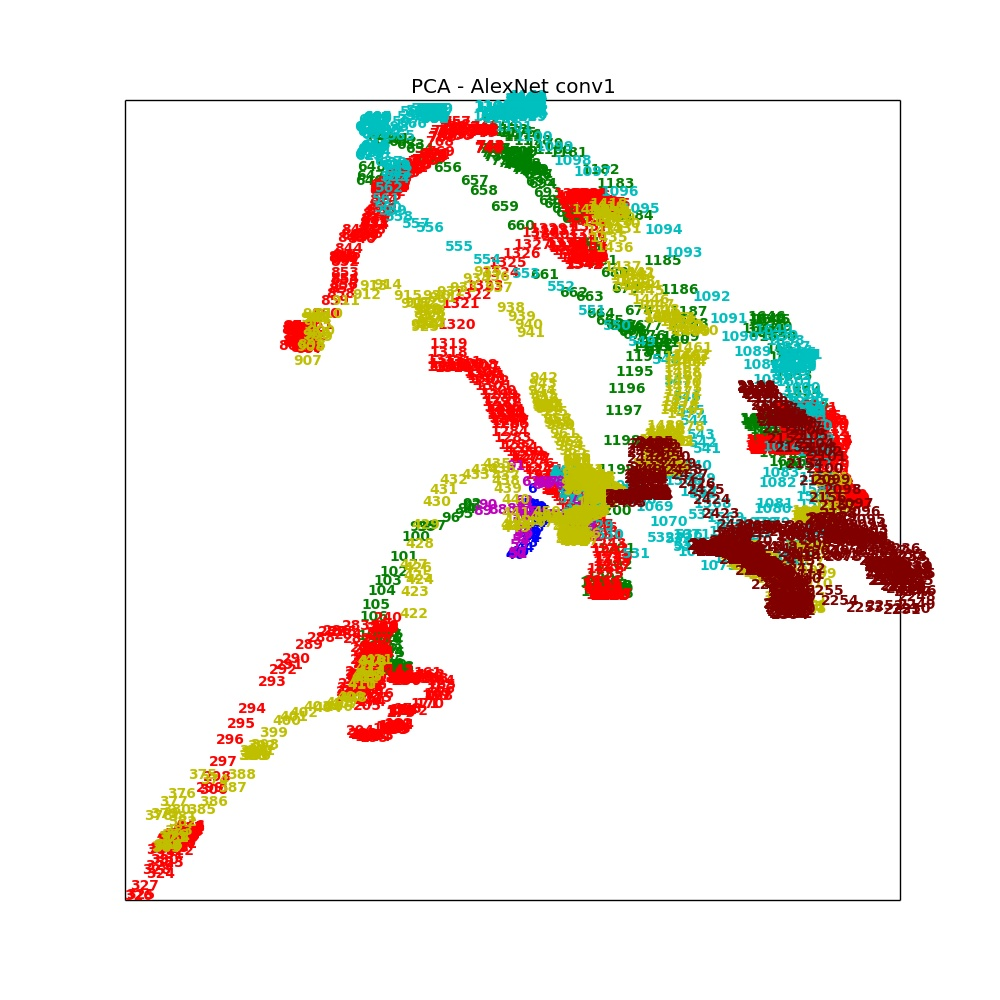
\includegraphics[width=\columnwidth]{figures/E5cap2_AlexNet_conv1_pca.jpg}
\caption{\todo{Fix image with more details, remove frame numbers and add points} \label{fig:imgtraj}}
\end{figure}

\section{Visual Featurization}
\begin{enumerate}

\item Describe goals

\begin{enumerate}
\item Spatially \& Scale invariant features
\item Key in on primitives
\end{enumerate}

\item Describe different ways that you can get visual features
\begin{enumerate}
\item Deep features from Convolutional Neural Networks
\begin{enumerate}
\item Pre-trained Architectures (VGG, AlexNet, C3D)
\item Encoding
\item Dimensionality-reduction and Correlation
\end{enumerate}
\item Tracking with Optical Flow
\item HOG
\item SIFT
\item PCA on RGB Images LOL \\
Need to show Figure with PCA? on all of them 
\end{enumerate}

\item Describe what we did and our methodology

\item Pre-processing
\begin{itemize}
\item Background subtraction
\begin{itemize}
\item A OpenCV built-in background subtraction algorithm was applied on each frame before pushing through the CNN. The algorithm was a Gaussian Mixture-based Background/Foreground Segmentation algorithm. It was introduced in the paper "An improved adaptive background mixture model for real-time tracking with shadow detection" by P. KadewTraKuPong and R. Bowden in 2001.
\end{itemize}

\item Cropping \& Scaling
\begin{itemize}
\item I cropped all frames by equal amounts to capture only the workspace where most of the robot manipulation happened. Then, they were rescaled to 640 x 480 dimensions. All pre-processing happened with ffmpeg.
\end{itemize}

\end{itemize}


\end{enumerate}
\section{Latent State $H_t$}
Describe the process of linking kinematics and video (PCA, CCA, etc.).
If we apply any VLAD or encoding, or batching, describe it here:

\begin{itemize}
\item Encoding - Current Status
\begin{itemize}
\item So I've implemented the following encoding method- Latent Content Descriptors (LCD) + VLAD. However, initial results weren't great and I need to see how it performs on milestones clustering.
\end{itemize}


Vector of Locally Aggregated Descriptors (VLAD) image encoding as proposed by \cite{jegou2010aggregating} is a method a feature encoding and pooling method, similar to Fisher vectors. VLAD encodes a set of local feature descriptors $I=(x_1,\ldots,x_n)$ extracted from an image using a codebook $\mathrm{C} = \{c_1, \ldots, c_m \}$ built using a clustering method such as Gaussian Mixture Models (GMM) or K-means clustering.


VLAD was shown to perform better than Fisher vectors and average pooling for encoding multiple frames~\cite{xu2014discriminative}.

\item Temporal Batching - Current Status
\begin{itemize}
\item While batching is supposed to help in video analysis , I've seen good separation of clusters (PCA on conv features) with just individual frames without clustering... I think I need to look into this more and need to test it out with milestones clustering.
\end{itemize}

\end{itemize}

\section{Clustering}
Describe the clustering procedure--refer to ISRR when needed.


\begin{figure*}[!t]
\centering
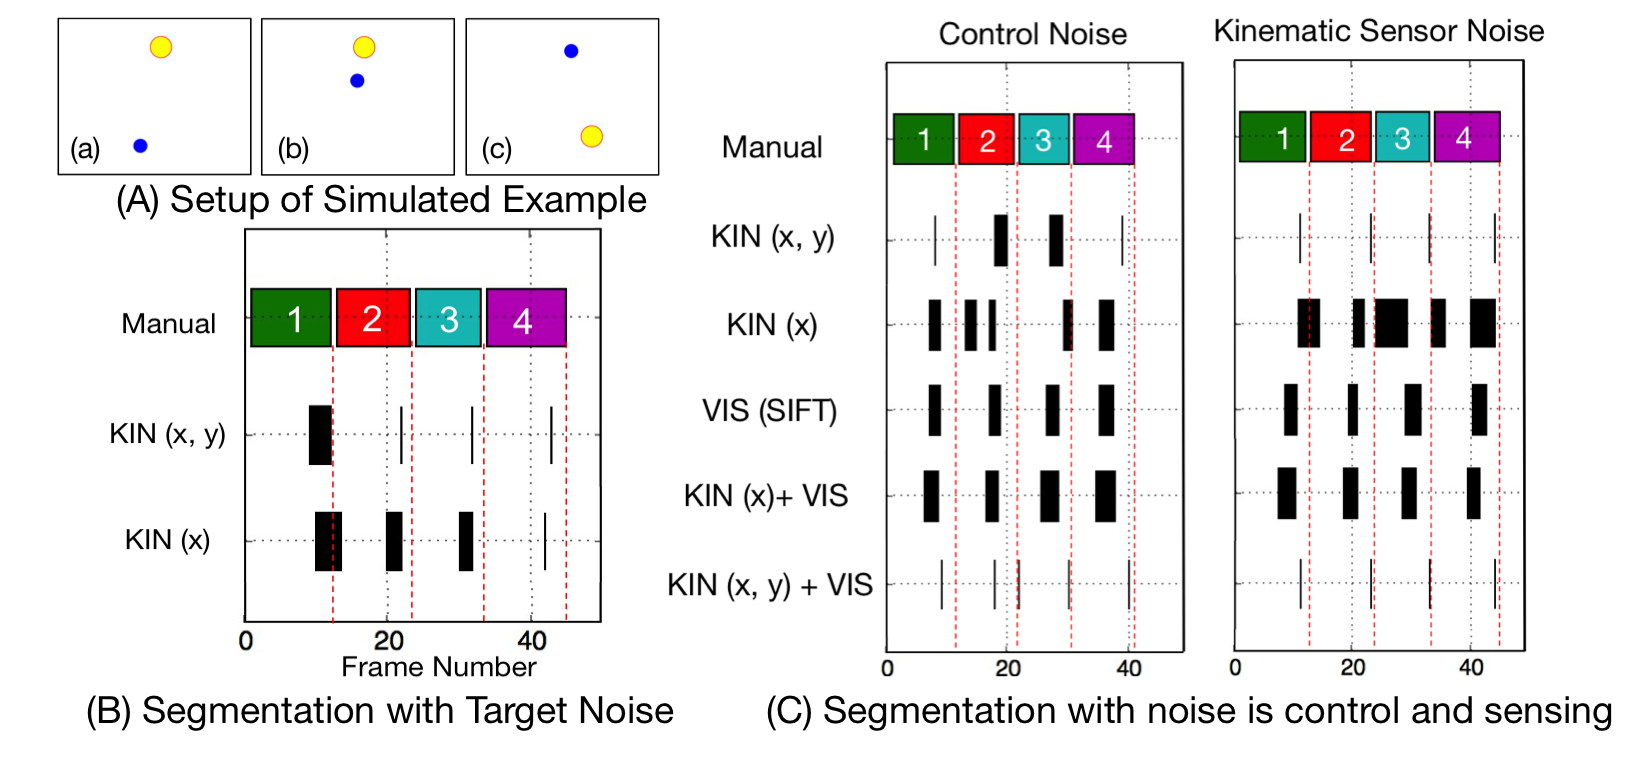
\includegraphics[width=0.8\linewidth]{figures/toyEx}
\caption{Each row is a sequence of transitions represented by blocks. The width of every block represents the confidence interval conveying the length of transition, with some transitions being sharp while others are longer.}
\label{fig:toyEx}
\vspace{-15pt}
\end{figure*}
\section{Results}
\subsection{Exp1. End-to-end result with some task}

\begin{enumerate}
\item Show that clusters are sensible and align with some intuitive criteria e.g., surgemes
\end{enumerate}

\subsection{Exp2. Does Vision Help}

\begin{enumerate}
\item Remove visual features and show that clusters degrade
\end{enumerate}

\subsection{Exp3. Parameter Search}

\begin{enumerate}
\item Describe our eval procedure and how we arrived at the architecture we did.
\end{enumerate}

\subsection{Exp4. Robustness}
\begin{enumerate}
\item Add noise or corrupt images and test to see how robust the segmentations we learn are.
\end{enumerate}


\subsection{Discussion}
\begin{enumerate}
\item How successful was our unsupervised approach in learning meaningful segmentations
\item RGB videos vs. RGB-D videos
\end{enumerate}


\section{Conclusion}
Summarize framework and results.


\bibliographystyle{IEEEtranS}
\bibliography{deepP2P}

\end{document}
